\documentclass{article}

\newcommand*{\plogo}{\fbox{$\mathcal{PL}$}}

\usepackage{indentfirst}
\usepackage{anysize}
\usepackage{graphicx}
\usepackage{subfigure}
\usepackage{array}
\usepackage{makecell}
\usepackage{CJK}

\usepackage{fancyhdr}
\pagestyle{fancy}
%\usepackage[colorlinks=true,linkcolor=black,citecolor=magenta,urlcolor=red]{hyperref}
%\usepackage[all]{hypcap}

\linespread{1.2}


\marginsize{3cm}{3cm}{1cm}{1cm}
\setlength{\parindent}{2em}

\newcolumntype{L}[1]{>{\vspace{0.5em}\begin{minipage}{#1}\raggedright\let\newline\\
\arraybackslash\hspace{0pt}}m{#1}<{\end{minipage}\vspace{0.5em}}}
\newcolumntype{R}[1]{>{\vspace{0.5em}\begin{minipage}{#1}\raggedleft\let\newline\\
\arraybackslash\hspace{0pt}}m{#1}<{\end{minipage}\vspace{0.5em}}}
\newcolumntype{C}[1]{>{\vspace{0.5em}\begin{minipage}{#1}\centering\let\newline\\
\arraybackslash\hspace{0pt}}m{#1}<{\end{minipage}\vspace{0.5em}}}

%使得图片显示对应章节
\renewcommand\thefigure{\thesection.\arabic{figure}}
\makeatletter
\@addtoreset{figure}{section}
\makeatother


\begin{document}
\begin{CJK}{UTF8}{gbsn}
%页眉、页脚设置
\lhead{
	\setlength{\unitlength}{1mm}
        \begin{picture}(0,0)
        \put(0,0){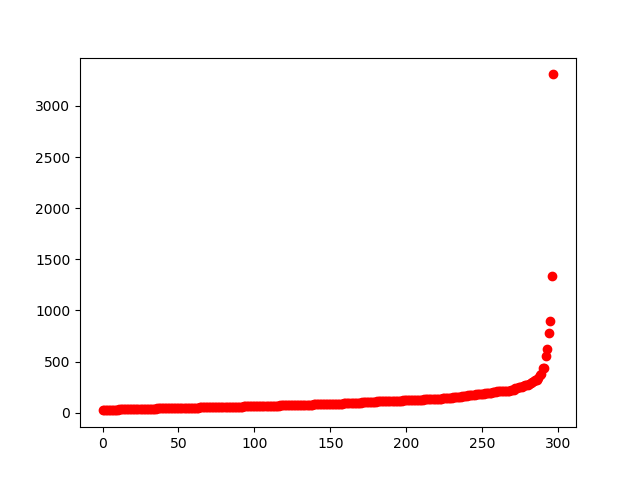
\includegraphics[width=0.7cm]{1.jpg}}
        \end{picture}
}
\chead{}
\rhead{\bfseries DAM-2018}
\lfoot{\itshape Tongji University}
\cfoot{\thepage}
\rfoot{\itshape School of Software Engineering}
\renewcommand{\headrulewidth}{0.4pt}
\renewcommand{\footrulewidth}{0.4pt}

\newcommand*{\titleGP}{\begingroup % Create the command for including the title page in the document
\centering % Center all text
\vspace*{\baselineskip} % White space at the top of the page

\rule{\textwidth}{1.6pt}\vspace*{-\baselineskip}\vspace*{2pt} % Thick horizontal line
\rule{\textwidth}{0.4pt}\\[\baselineskip] % Thin horizontal line

{\LARGE 超市数据的频繁项集挖掘 -- a问分析文档
 \\ \vspace{2em} \begin{large} 数据分析与数据挖掘 \end{large}}\\[0.2\baselineskip] % Title

\rule{\textwidth}{0.4pt}\vspace*{-\baselineskip}\vspace{3.2pt} % Thin horizontal line
\rule{\textwidth}{1.6pt}\\[\baselineskip] % Thick horizontal line

\scshape % Small caps
%周一  饶卫雄老师 \\[\baselineskip] % Tagline(s) or further description
DAM COURSE, SPRING 2018\par % Location and year

\vspace*{2\baselineskip} % Whitespace between location/year and editors

 BY \\[\baselineskip]
{\Large 1552674 李\quad 源  \par} % Editor list


\vspace{23em}
\begin{figure}[!h]
\begin{center}
  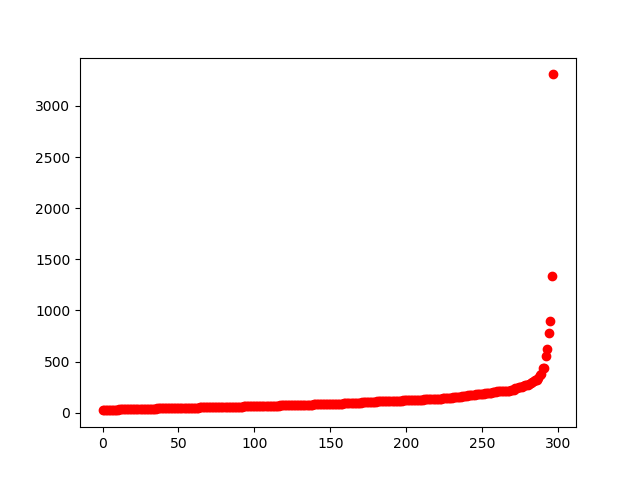
\includegraphics[width = 0.2\textwidth]{1.jpg}	
\end{center}
\end{figure}
\vfill

{\itshape Tongji University \\ School of Software Engineering \par} % Editor affiliation
\endgroup}

\titleGP % This command includes the title page
\thispagestyle{empty}
\clearpage


\section{trade\_new.csv文件数据代码运行结果}
\subsection{数据预处理耗时}

针对ai问的数据预处理时间如下:
\begin{figure}[!h]
\begin{center}
  \includegraphics[width = 0.9\textwidth]{ai.png}	
\end{center}
\end{figure}

针对aii问的数据预处理时间如下:
\begin{figure}[!h]
\begin{center}
  \includegraphics[width = 0.9\textwidth]{aii.png}	
\end{center}
\end{figure}

\subsection{ai问针对三个字段的频繁集求取情况}
\subsubsection{频繁集个数}
针对pluno、dptno、bndno字段,在2、4、8、16、32、64分别作为最小支持度时,频繁集个数:

\begin{figure}[!h]
\begin{center}
  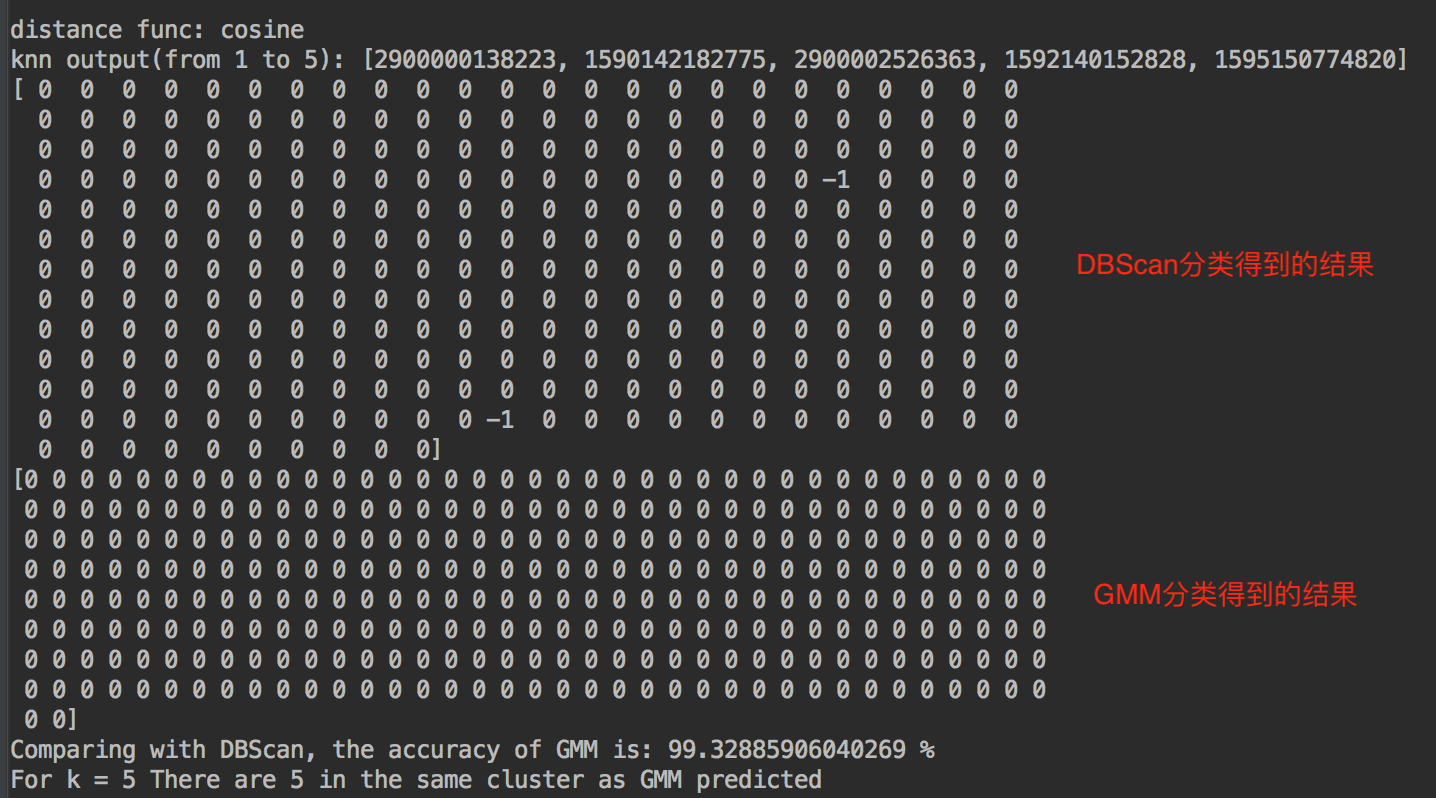
\includegraphics[width = 0.9\textwidth]{2.png}	
\end{center}
\end{figure}

\clearpage
\subsubsection{运行时间}
针对pluno、dptno、bndno字段,在2、4、8、16、32、64分别作为最小支持度时,运行时间:
\begin{figure}[!h]
\begin{center}
  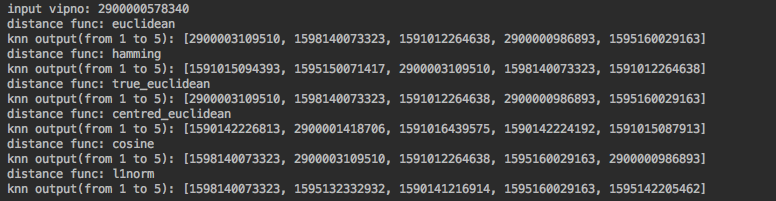
\includegraphics[width = 0.9\textwidth]{3.png}	
\end{center}
\end{figure}

\subsubsection{具体输出}
针对pluno、dptno、bndno字段,在16作为最小支持度时,使用SPMF包获得的输出结果:

pluno字段:
\begin{figure}[!h]
\begin{center}
  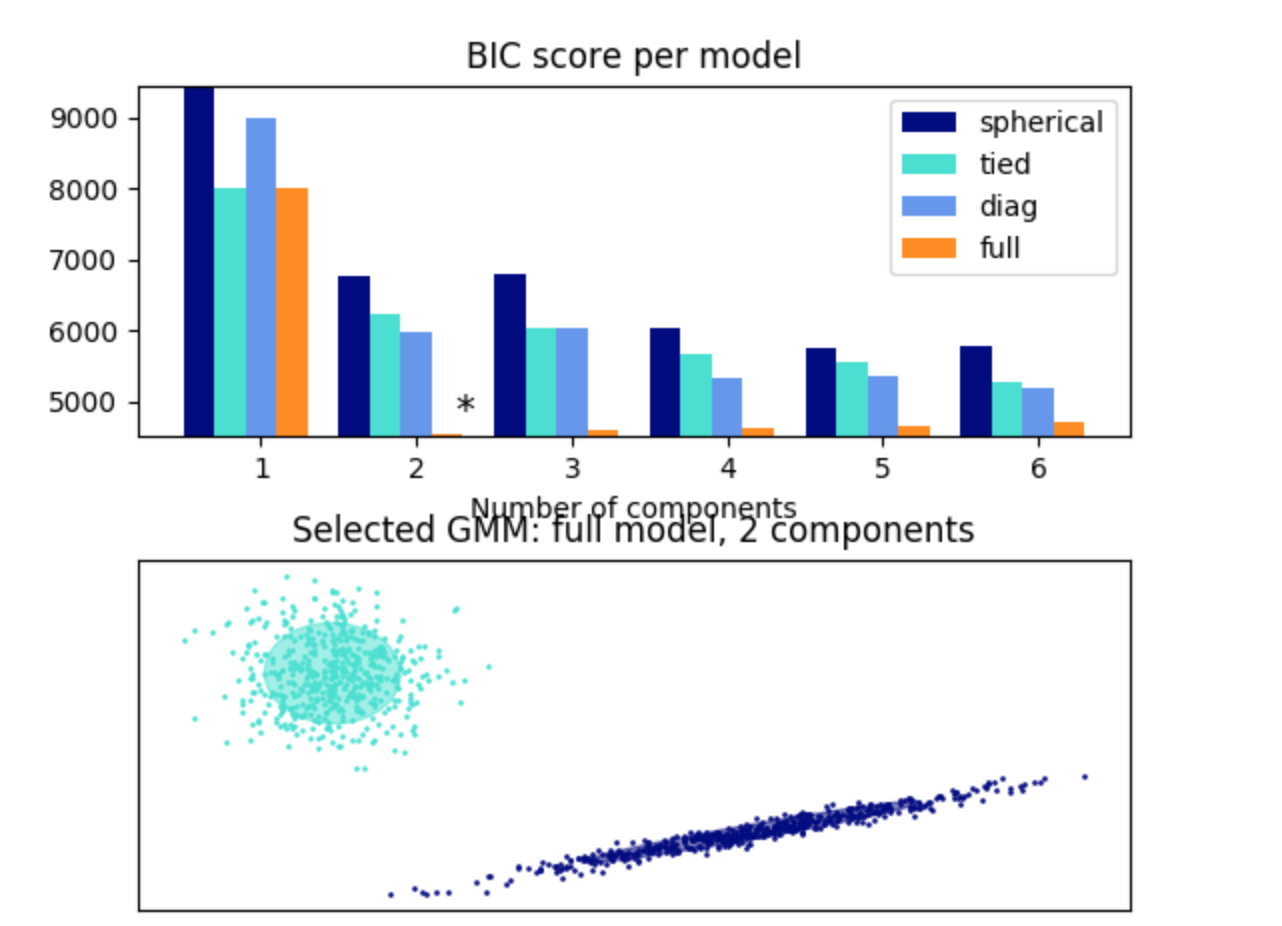
\includegraphics[width = 0.8\textwidth]{4.png}	
\end{center}
\end{figure}

dptno字段:
\begin{figure}[!h]
\begin{center}
  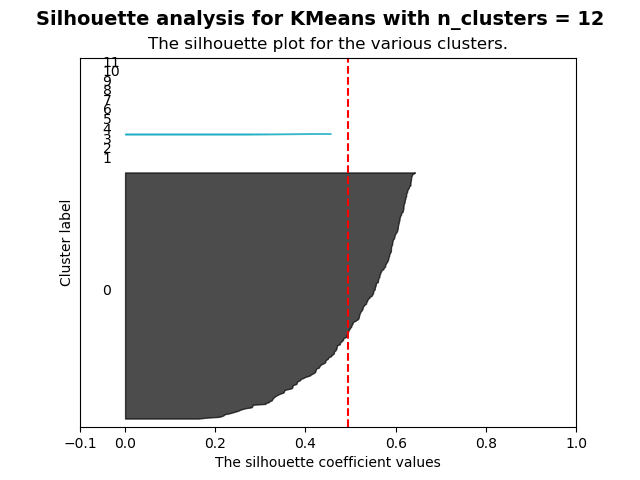
\includegraphics[width = 0.8\textwidth]{5.png}	
\end{center}
\end{figure}

bndno字段:
\begin{figure}[!h]
\begin{center}
  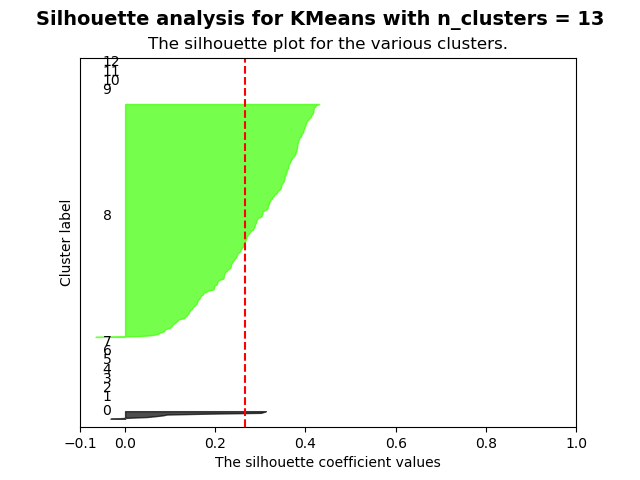
\includegraphics[width = 0.8\textwidth]{6.png}	
\end{center}
\end{figure}

\clearpage

\subsection{aii问针对三个字段的频繁集求取情况}
\subsubsection{频繁集个数}
针对pluno、dptno、bndno字段,在2、4、6、8、10分别作为最小支持度时,频繁集个数:

\begin{figure}[!h]
\begin{center}
  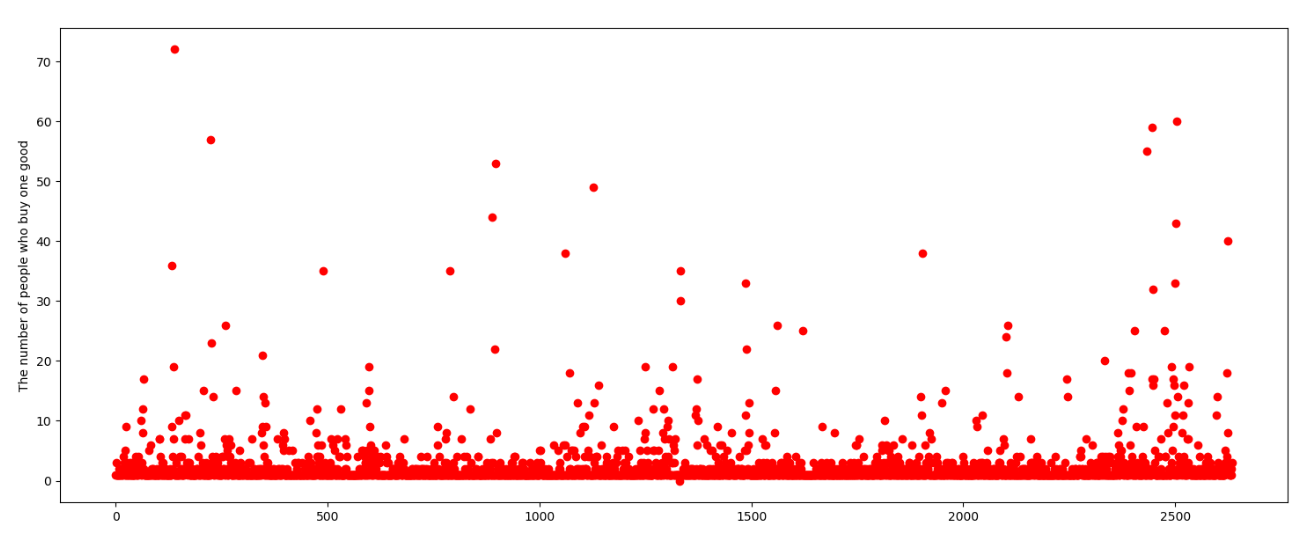
\includegraphics[width = 0.9\textwidth]{8.png}	
\end{center}
\end{figure}


\subsubsection{运行时间}
针对pluno、dptno、bndno字段,在2、4、6、8、10分别作为最小支持度时,运行时间:
\begin{figure}[!h]
\begin{center}
  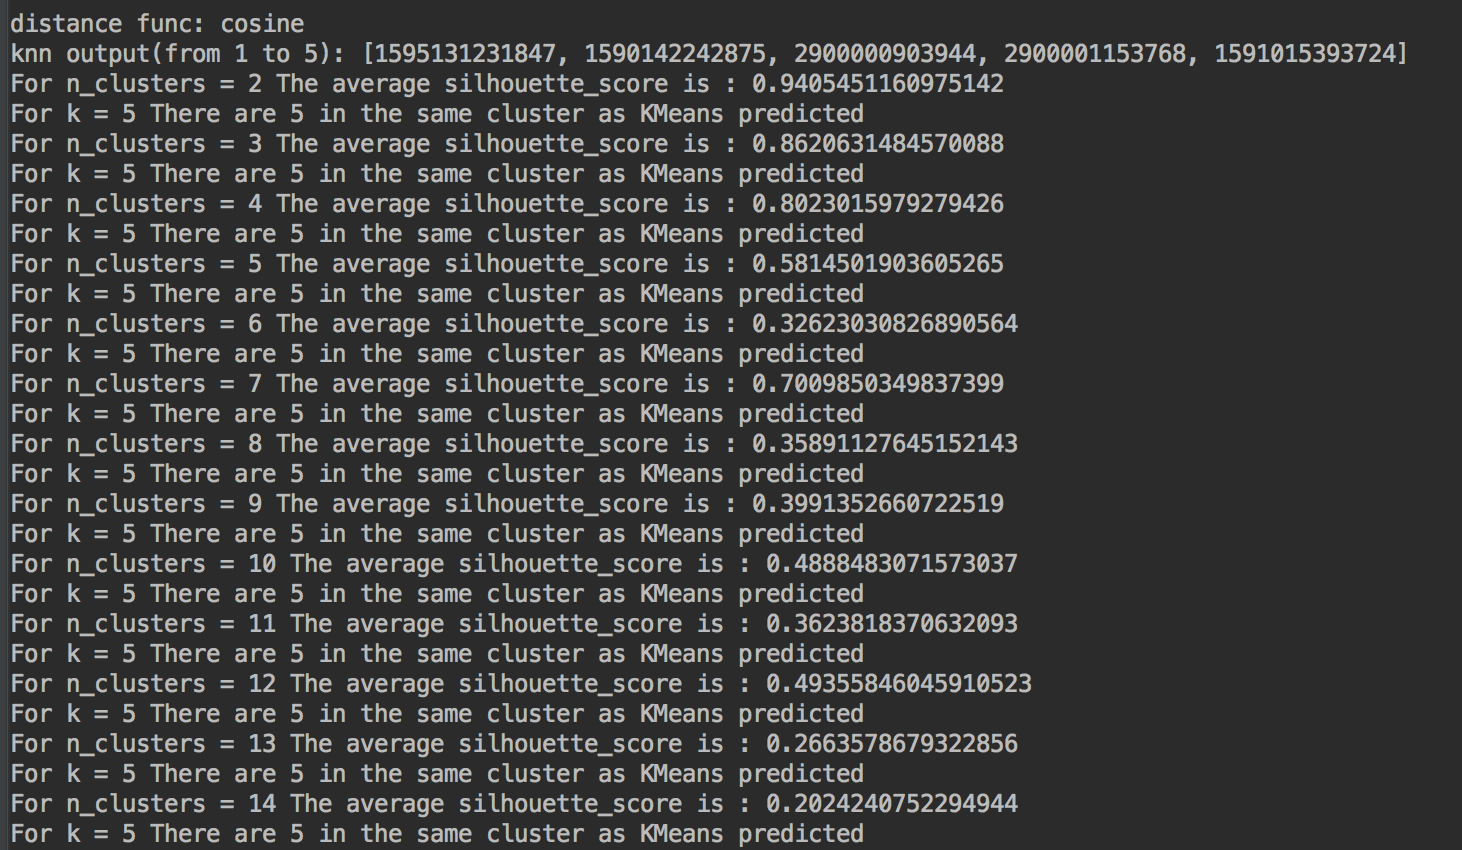
\includegraphics[width = 0.9\textwidth]{7.png}	
\end{center}
\end{figure}

\subsubsection{具体输出}
针对pluno、dptno、bndno字段,在8作为最小支持度时,使用SPMF包获得的输出结果:


pluno字段:
\begin{figure}[!h]
\begin{center}
  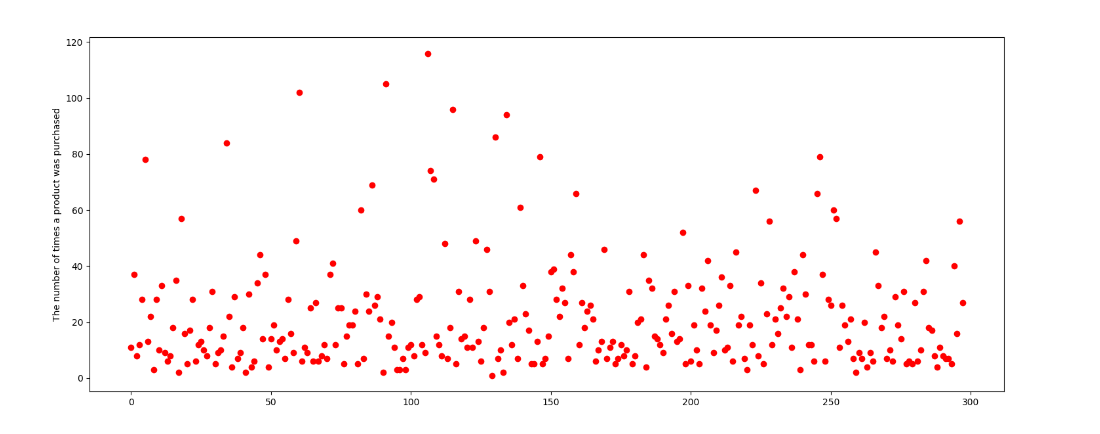
\includegraphics[width = 0.8\textwidth]{9.png}	
\end{center}
\end{figure}

dptno字段:
\begin{figure}[!h]
\begin{center}
  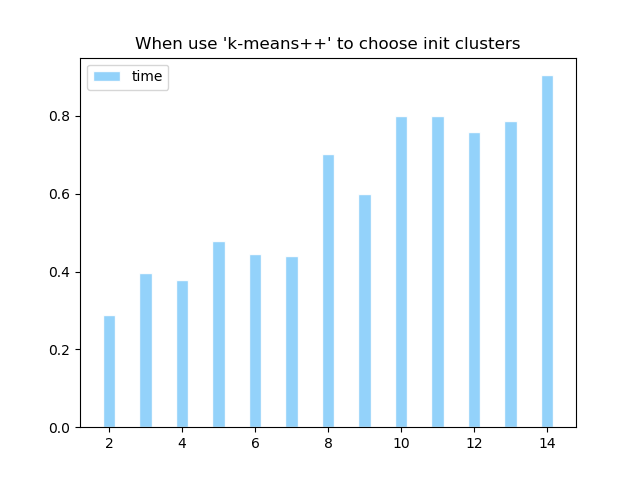
\includegraphics[width = 0.8\textwidth]{10.png}	
\end{center}
\end{figure}

bndno字段:
\begin{figure}[!h]
\begin{center}
  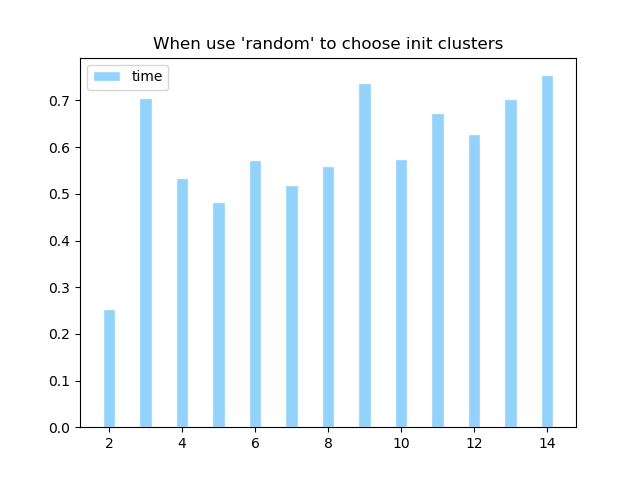
\includegraphics[width = 0.8\textwidth]{11.png}	
\end{center}
\end{figure}

总的来说,除了对应dptno字段在最小支持度为2的时候,所耗时间较长之外,其他的运行时间都在100ms之内,由此可见FP-growth算法的效率是比较高的。当然也因为我使用的SPMF包是基于Java做的实现。在最后的性能比较时,我会将基于Python实现的FP-growth算法与基于Java的实现进行对比。

具体的输出在这里选择了一个最小支持度对应的详细情况,作为展示。

\textbf{所有的结果都是进行了“对每个VIPNO对交易数据进行分组,按照sldat字段为标准取每个用户最早60\%的交易记录作为训练数据”这样的操作。}


\section{trade.csv文件数据代码运行结果}

\subsection{数据预处理耗时}

针对ai问的数据预处理时间如下:
\begin{figure}[!h]
\begin{center}
  \includegraphics[width = 0.7\textwidth]{14.png}	
\end{center}
\end{figure}

针对aii问的数据预处理时间如下:
\begin{figure}[!h]
\begin{center}
  \includegraphics[width = 0.7\textwidth]{15.png}	
\end{center}
\end{figure}

\clearpage
\subsection{ai问针对三个字段的频繁集求取情况}

\subsubsection{频繁集个数}
针对pluno、dptno、bndno字段,在2、4、8、16、32、64分别作为最小支持度时,频繁集个数:

\begin{figure}[!h]
\begin{center}
  \includegraphics[width = 0.9\textwidth]{16.png}	
\end{center}
\end{figure}


\subsection{aii问针对三个字段的频繁集求取情况}

\subsubsection{频繁集个数}
针对pluno、dptno、bndno字段,在2、4、6、8、10分别作为最小支持度时,频繁集个数:

\begin{figure}[!h]
\begin{center}
  \includegraphics[width = 0.9\textwidth]{17.png}	
\end{center}
\end{figure}


\section{分析讨论}
这里主要针对数据的预处理、最小支持度阈值的合理性、FP-growth的优劣和两份数据的差异性来进行分析讨论。

\subsection{数据的预处理}
在题目中有这样一个要求:\textbf{要求对每个VIPNO对交易数据进行分组,按照sldat字段为标准取每个用户最早60\%的交易记录作为训练数据。}这里利用Python中的Pandas包可以很轻松的实现。大概步骤如下:

1)利用Pandas包将数据读入之后,重新设置vipno、sldat字段分别为一级、二级索引。

2)利用$Pandas.DataFrame.sort\_index()$函数根据索引排序。

3)然后重新设置索引为vipno(这样做的好处在于能够加快之后通过索引取值的性能)。

4)依次取出每一个vipno的值,前60\%做训练集,后40\%做测试集。

5)最后根据uid或者vipno(分别对应ai问和aii问)进行合并。这里合并可以利用Python中的字典来做,写起来比较方便。

总的来说,Pandas这个包来处理数据挺方便的,但也有一些不方便的地方,在这次做预处理的时候也遇到了一些坑。大概整理如下:

首先是如果读取$Pandas.DataFrame$中的一行数据,Pandas会自动地帮你转成$Series$格式,这点不同于$numpy.ndarray$,这样就可能出现部分函数不能使用(比如$Pandas.Series$就没有$as\_matrix()$这个函数)、数据长度难以判断(针对$len$函数,$Pandas.DataFrame$是返回的有多少行,而$Pandas.Series$是返回有多少个单一数据,因为它只有一行)等情况,需要单独考虑。

每一列字段的数据格式也需要考虑。Panda是在从csv文件读取数据的时候,会根据这一列字段的数据情况,将数据类型设定成Pandas自身认为“合理”的一种类型,比如$int$、$float$等等(如果直接用csv包,那么读出来的都是$str$格式,当然你要是用默认的$open$函数,那就一整行就是一个字符串)。有利有弊吧,有时候其实这样做会很“蠢”。在我处理bndno字段的时候,Pandas就帮我将这个字段转成了$float$格式,而且对于空的数据补成了$float('nan')$。我还需要对这些数据单独处理一下,比较烦。

\subsection{最小支持度阈值的合理性}

首先定义一下频繁项集的概念:

1)我们称$I={i_{1},i_2,...,i_m}$为项(Item)的集合,$D=\{T_1,T_2,...,T_n\},i\in[1,n]$为事务数据集(Transaction Data Itemsets),事务$T_i$由$I$中若干项组成。

2)设$S$为由项组成的一个集合,$S={i| i \in I}$,简称项集(Itemset)。包含$k$个项的项集称为k-项集。

3)$t$为一条事务, 如果$S \subset t$, 则称事务$t$包含$S$。

4)那么$S$的支持度:

\begin{equation}
sup(S) = (S)/(D) * 100\%
\end{equation}

5)若$S$的支持度 ≥ 给定最小支持度,称$S$为频繁项集(Frequent Itemset)。

在作业要求中,最小支持度(minsup)的阈值分别为2、4、8、16、32、64,和2、4、6、8、10。都是绝对的值。然而我们可以发现,SPMF在设置最小支持度是按照百分比来的。实际上这是有道理的。我们可以计算出64和10这两个最大的阈值转换成百分比之后应该分别为:2.33\%和2.06\%,并不算很高;而当阈值取2、4的时候,转换成百分比就十分的小了,最先我觉得,这样获取到的频繁项集的说服力并不大。一般通常的最小支持度取10\%、20\%、30\%、40\%、50\%、60\%... 这样的增长性数组可能更加具有普适性。

但是,最小支持度的设置也需要考虑到具体的数据。对于本次作业的数据,如果最小支持度设置较大的话,我们会发现根本找不到频繁项集了。总的来说,最小支持度取16、32和6、8的时候,针对本次的数据相对比较合理。

阈值定的过小的一个问题,就是可能会导致输出的频繁项集太多,比如对于aii问的dptno字段,当阈值为2时候,有300余万个频繁集,其实对于推荐算法、关联规则等的推到已经没有太大的意义了。

\subsection{FP-growth的优劣}
FP-growth算法将事务数据库$D$有效地压缩成小存储空间的数据结构, 与之前我们学到的Apriori算法相比,解决了多次扫描事务数据库的这个缺陷,只需对事务数据库进行二次扫描,我觉得可以理解成是利用递归模式的策略,这样候选集就会比较少,大大降低了算法的时间复杂度。

不过FP-growth也存在两个问题:

1)算法在挖掘大型数据集时如果由原数据库得到的FP-tree的分支很多, 而且分支长度很长时, 该算法将需要构造出数量巨大的条件FP-tree, 不仅费时而且要占用大量的空间。

2)算法在挖掘频繁模式过程中存在性能瓶颈: 由于该算法要递归生成条件数据库和条件FP-tree, 而条件FP-tree需要自顶向下生成, 频繁模式的挖掘需要自底向上处理, 在挖掘时需要反复地搜索 FP-tree, 这就需要更多的指针, 所以内存开销大。看具体的输出就能发现,跑一次算法消耗的内存在80mb左右。

\subsection{两份数据的差异性}
具体结果在前面有详细展示,这里做一个简单说明。

我把两份数据做了一个简单比较,可以发现trade\_new.csv的数据包含了大部分旧的trade.csv数据。这个在运行结果上也可以体现出来。下面两个图分别是trade\_new.csv和trade.csv的数据对于ai问的pluno字段,支持度前十的频繁项集:

\begin{figure}[!h]
\begin{center}
  \includegraphics[width = 0.6\textwidth]{18.png}
  \caption{trade\_new.csv}	
\end{center}
\end{figure}

\begin{figure}[!h]
\begin{center}
  \includegraphics[width = 0.6\textwidth]{19.png}	
  \caption{trade.csv}
\end{center}
\end{figure}

我们可以发现,其前十的pluno字段都比较相近,但是对应的支持度会存在一定的差异。进一步比较其她的频繁项集,再加上两者数据的重合度,我应该可以认为,这两份数据是都来自于同一个地区的一家或者几家超市的购买数据。在c问的中,我会进一步从预测方面对两者数据进行比较。

\section{性能比较}

首先我比较基于Java实现的SPMF包和基于Python实现的enaeseth包、evandempsey包三者运行FP-growth算法的效率,结果如下:

\clearpage
\begin{figure}[!h]
\begin{center}
  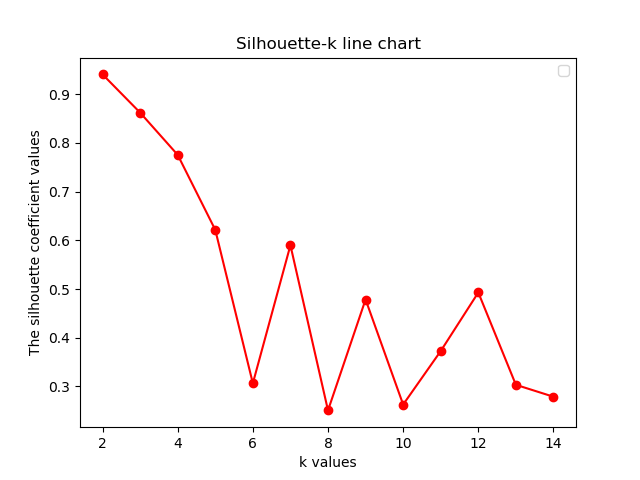
\includegraphics[width = 0.8\textwidth]{12.png}	
\end{center}
\end{figure}


很显然的,基于Java性能实现的包要比Python包计算时间更好,不过Java主要在于灵活性相对Python要差一些,没有Python那些奇葩特性, 灵活性不足。都有优劣吧,不过现在来说,当前流行的一些开源的机器学习包使用Python实现的会更多一些,当然Python易于上手也是一个原因。

之后我比较了FP-growth算法和Apriori算法之间的性能,

\begin{figure}[!h]
\begin{center}
  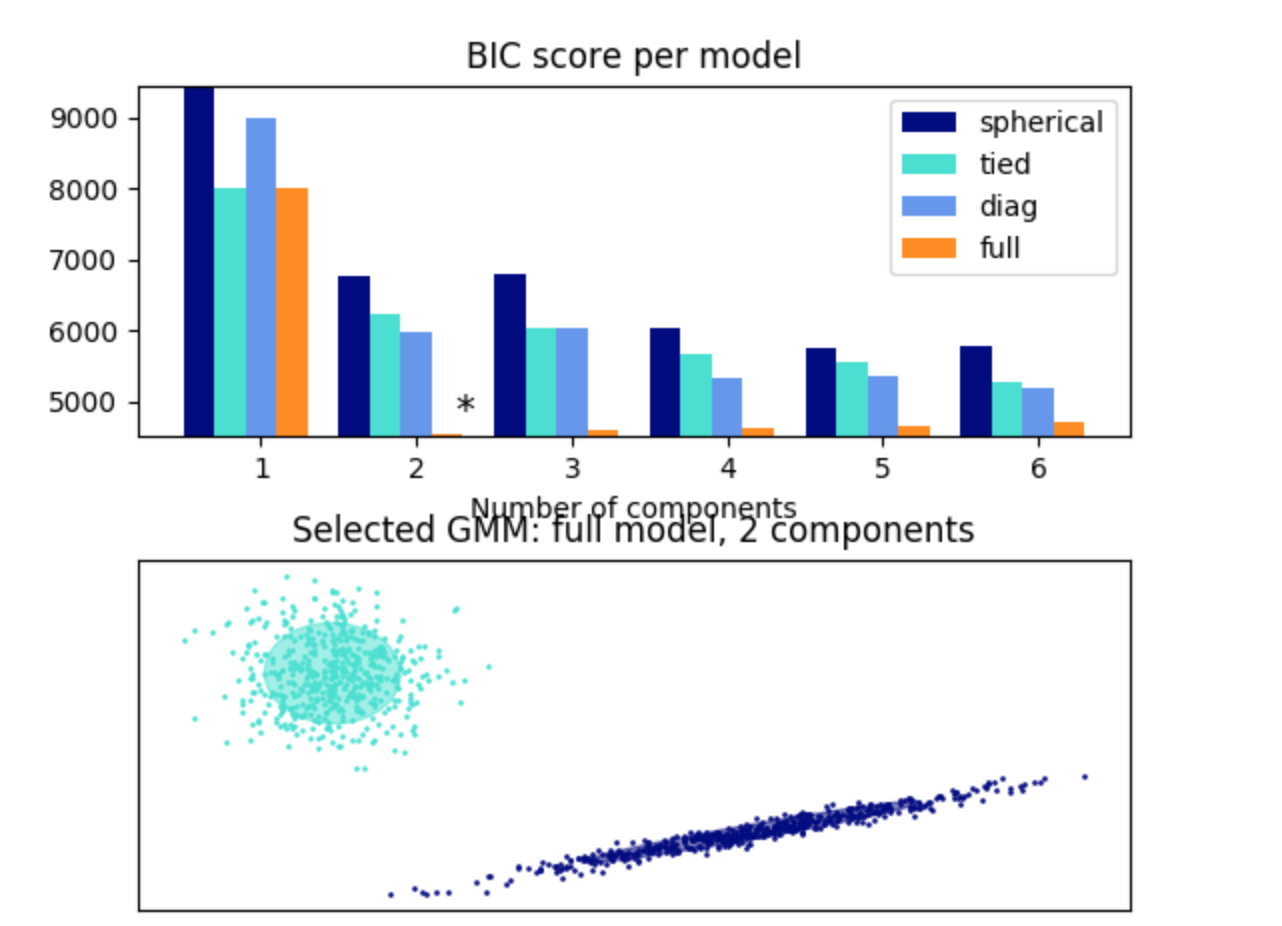
\includegraphics[width = 0.8\textwidth]{4.png}	
\end{center}
\end{figure}

\begin{figure}[!h]
\begin{center}
  \includegraphics[width = 0.8\textwidth]{13.png}	
\end{center}
\end{figure}

很明显在时间和内存上,FP-growth算法都比Apriori算法要好,其原因在前文的分析中有一个详细地描述,这里就不再重复了。

\end{CJK}
\end{document}

